\documentclass[12pt, a4paper]{article}

\usepackage[T2A]{fontenc}
\usepackage[utf8]{inputenc}
\usepackage[english, russian]{babel}
\usepackage{amssymb}
\usepackage{amsfonts}
\usepackage{amsmath}
\usepackage{mathtext}

\usepackage{comment}
\usepackage{geometry}
\geometry{left=1cm, right=1cm, top=2cm, bottom=2cm}

\usepackage{graphicx}
\usepackage{tikz}

\usepackage{wrapfig}
\usepackage{fancybox,fancyhdr}
\sloppy

\setlength{\headheight}{28pt}

\newcommand{\head}[4]
{
	\fancyhf{}
	\pagestyle{fancy}
	\chead{#3, #4}

	\begin{center}
	\begin{large}
	#1 \\
	\textit{#2} \\
	\end{large}
	\end{center}

}

\begin{document}

\head{IX Республиканская студенческая предметная олимпиада по направлению \\ <<Математика>>}{13 апреля 2017}{Казахстанский филиал МГУ имени М. В. Ломоносова}{г. Астана}

\begin{enumerate}

\item (Абдикалыков А.)

Пусть $S=\displaystyle\sum\limits_{n=1}^{\infty}{\frac{T_n}{2^n}}$. Тогда
$$
\sum\limits_{n=1}^{\infty}{\frac{T_{n+1}}{2^n}}=2\cdot \sum\limits_{n=1}^{\infty}{\frac{T_{n+1}}{2^{n+1}}}=2\cdot \left(S-\frac{T_1}{2^1}\right)=2S-1,
$$
$$
\sum\limits_{n=1}^{\infty}{\frac{T_{n+2}}{2^n}}=4\cdot \sum\limits_{n=1}^{\infty}{\frac{T_{n+2}}{2^{n+2}}}=4\cdot\left(S-\frac{T_1}{2^1}-\frac{T_2}{2^2}\right)=4S-3,
$$
\begin{multline*}
\sum\limits_{n=1}^{\infty}{\frac{T_{n+3}}{2^n}}=8\cdot \sum\limits_{n=1}^{\infty}{\frac{T_{n+3}}{2^{n+3}}}=\\
=8\cdot\left(S-\frac{T_1}{2^1}-\frac{T_2}{2^2}-\frac{T_3}{2^3}\right)=8S-7.
\end{multline*}

Так как по условию $T_{n+3}=T_{n+2}+T_{n+1}+T_n$, то $$8S-7=4S-3+2S-1+S,$$ откуда следует $S=3$.

\item (Абдикалыков А.)

Пусть $k$-ичная запись простого числа $p$ для некоторого $k>1$ выглядит как $\overline{a_0a_1\hdots a_{k-1}}$, где $(a_0, a_1, \hdots, a_{k-1})$ --- некоторая перестановка цифр $(0, 1, \hdots, k-1)$. Тогда
$$
p = a_0\cdot k^{k-1} + a_1\cdot k^{k-2}+\hdots+a_{k-1}\cdot k^0 \equiv
$$
$$
= a_0+a_1+\hdots+a_{k-1} \pmod {(k-1)}.
$$
Поскольку сумма всех цифр равна $k(k-1)/2$, то можно сделать вывод, что число $p$ делится на $(k-1)/2$, если $k$ нечётно и на $k-1$, если $k$ чётно. Учитывая, что $p\geqslant k^{k-1}>k-1$ --- простое число, заключаем, что $k$ должно удовлетворять совокупности соотношений
$$
\left[
\begin{matrix}
\frac{k-1}{2}=1,& k = 2l+1,\\
k-1=1, & k = 2l.\\
\end{matrix}
\right.
$$
Таким образом, $k=2$ или $k=3$, а значит, достаточно перебрать числа $10_2$, $102_3$, $120_3$, $201_3$, $210_3$. Простыми среди них являются только $2=10_2$, $11=102_3$ и $19=201_3$.

\item (Клячко А.)

а) Для любого элемента $x$ порядка 2 верно $x=x^{-1}$, поэтому
$$
(ab)^2=abab=aba^{-1}b^{-1},
$$
если $a^2=b^2=e$.

б) Аналогично, для любого элемента $x$ порядка 3 верно $x^2=x^{-1}$, поэтому
\begin{multline*}
(ab)^3=ababab=ab^4aba^4b=(ab^2)(b^2a)(ba^2)(a^2b)=\\
(ab^2)(b^2a)(ab^2)^{-1}(b^2a)^{-1},
\end{multline*}
если $a^3=b^3=e$.

\item (Баев~А.)

Обозначим через $F$ фокус параболы,  через $d$ директрису параболы. Рассмотрим произвольную касательную к параболе $l$ в произвольной точке $C$.

\begin{center}
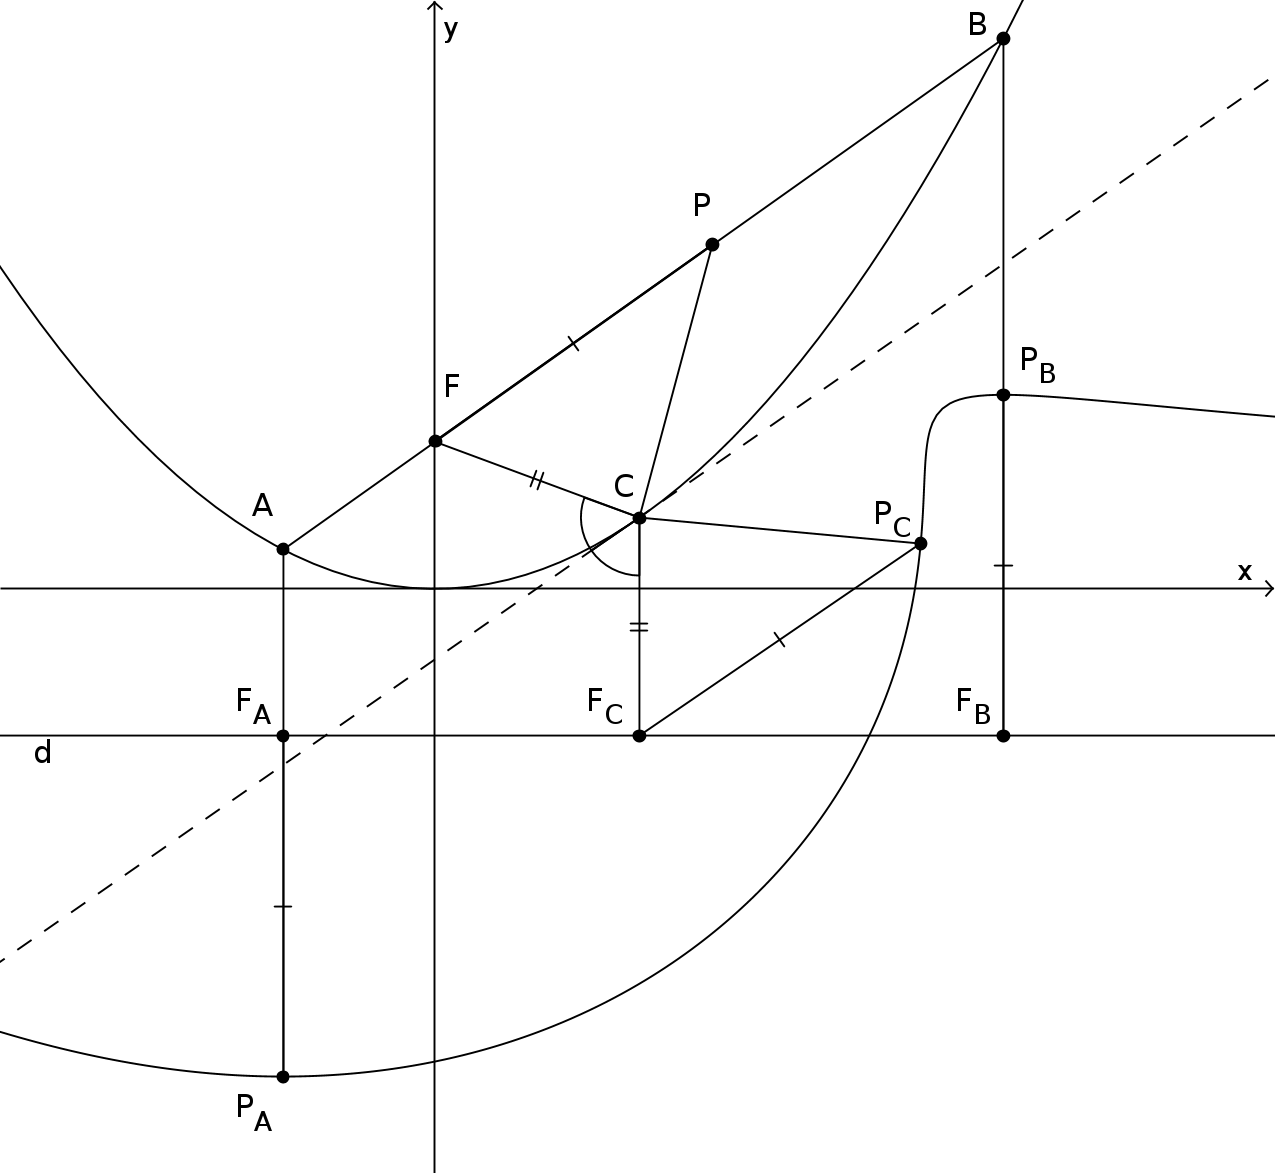
\includegraphics[scale=0.9]{pictures/2017-republic}
\end{center}

Свойство 1: точка $F_C$, симметричная $F$ относительно $l$, лежит на директрисе $d$. 

Из определения параболы: $FC = F_CC$. Из оптического свойства параболы $\angle(FC; l) = \angle(l; F_CC)$. Получаем, что $l$ --- ось симметрии для отрезков $FC$ и $F_CC$. 

Свойство 2: $$ -\frac{1}{4} - FP \leqslant y(P_C)  \leqslant -\frac{1}{4} + FP,$$
где $y(P_C)$ --- ордината точки $P_C$.

Известна директриса данной параболы $y = -\frac{1}{4}$. Ордината точки $F_C$ равна $-\frac{1}{4}$. А точка $P_C$ находится на расстояния не более, чем $F_CP_C$ от директрисы. Осталось заметить, что с учетом свойства 1 треугольники $FCP$ и $F_CCP_C$ равны, то есть $F_CP_C = FP$.

Свойство 3:  $\displaystyle \max_{(x, y) \in S(P)} y = -\frac{1}{4} + FP$ и $\displaystyle \min_{(x, y) \in S(P)} y = -\frac{1}{4} - FP$. 

Максимум или минимум $y(P_C)$ в свойстве 2 достигается в том случае, если $P_CF_C$ перпендикулярно директрисе. Причем для максимума необходимо, чтобы $P_C$ и $C$ лежали по одну сторону от директрисы, а для минимума --- по разные стороны. То есть угол $CF_CP_C$ равен либо 0, либо $\pi$ (соответственно, угол $CFP$ равен либо 0, либо $\pi$). В качестве таких точек $C$ достаточно выбрать точки  пересечения $FP$ с параболой $A$ и $B$. Значит, оба равенства в свойстве 2 достигаются.

Свойство 4: геометрическим местом точек в пункте б) является окружность с центром в $F$ и радиусом $\frac{1}{4}$. Из свойства 3 следует, что $FP = F_BP_B = \frac{1}{4}$.

\item (Васильев А.)

Ответ: да, существует.

Можно привести множество примеров, но мы укажем самый простой:
$$
f(x) =
\begin{cases}
0, x \in [0, 1)\\
1, x = 1
\end{cases}
$$
Обозначив $\frac{i}{n}$ через $x_i$, имеем: $m_i = \inf_{x \in [x_{i-1}, x_i]} f(x) = 0$ для всех $i = \overline{1,n}$ и 
$$M_i = \sup_{x \in [x_{i-1}, x_i]} f(x) =\begin{cases} 
0, i = \overline{1, n-1} \\ 
1, i = n
\end{cases}
$$
Следовательно, $s_n(f) = 0$ и $S_n(f) = \frac{1}{n}$ для всех $n \in \mathbb{N}$. При этом $f$ интегрируема на $[0, 1]$, ряд $\displaystyle \sum_{n=1}^{\infty} 0$ сходится, а ряд $\displaystyle \sum_{n=1}^{\infty} \frac{1}{n}$ расходится.

\item (Высоканов Б., Клячко А.)

Обозначим через $n$ количество участников олимпиады и присвоим им номера от 1 до $n$. Пусть $a_{ij}$ --- количество решений, списанных $i$-ым участником у $j$-го, при этом полагаем $a_{ii} = 0$. Рассмотрим два случая:

1) $n = 2k$, $k \in \mathbb{N}$. Если $k = 1$, то доказательство тривиально. Пусть $k \leqslant 2$. Доказательство проведем от противного. Допустим, что, выгоняя любые $k$ человек из $2k$, мы никогда не достигнем требуемого. Тогда для любого $S' \subset S$, где $|S'| = k$ и $S = \{1, 2, ..., 2k \}$, имеем:
$$\sum_{\substack{i \in S' \\ j \in S \backslash S'}} \leqslant \frac{1}{4} \sum_{i, j \in S} a_{ij}.$$

Просуммируем эти неравенства по всем $S'$:
$$\sum_{S'} \sum_{\substack{i \in S' \\ j \in S \backslash S'}} a_{ij} \leqslant \frac{1}{4} \sum_{S'} \sum_{i, j \in S} a_{ij}.$$

Заметим, что каждое $a_{ij}$ при $i \neq j$ в сумме слева встретится ровно $C_{2k-2}^{k-1}$ раз, а в сумме справа --- ровно $C_{2k}^{k}$ раз. Разделив обе части неравенства на $\sum_{i, j \in S} a_{ij} > 0$, находим:
$$ C_{2k-2}^{k-1} \leqslant \frac{1}{4} C_{2k}^k,$$
что неверно, так как 
$$\frac{C_{2k}^{k}}{C_{2k-2}^{k-1}} = 2 \left( 2 - \frac{1}{k} \right) < 4.$$

2) $n = 2k + 1$, $k \in \mathbb{N}$. При $k = 1$ доказательство тривиально. При $k \geqslant 2$ рассуждаем аналогично 1), рассматривая все $S' \in S$ с условием $|S'| = k$ (при этом $S = \{1, 2, ..., 2k+1\}$).

\end{enumerate}

\end{document} 
